% Proposition 4: Quadratic Regret Bound (Condensed for Main Body)
% Full proof and details in Appendix~\ref{app:quadratic_proof}

\subsection{Theoretical Foundation: Quadratic Regret Bound}
\label{subsec:quadratic_regret}

We now provide theoretical justification for \textit{why} O/R predicts coordination success.

\begin{proposition}[Quadratic Regret Bound]
\label{prop:quadratic_regret}
Under standard assumptions (bounded discrete actions, sufficient samples per observation bin, action-matching coordination, non-degenerate variance, stationary symmetric policies), the coordination regret satisfies:
\begin{equation}
\text{Regret}(\pi) \leq C_m \cdot (\text{OR}(\pi) + 1)^2
\end{equation}
where $C_m$ is a characterized task-dependent constant. Lower O/R yields quadratically less regret.
\end{proposition}

\textbf{Intuition.} Coordination failures compound: when agent $i$ cannot predict agent $j$'s actions (high O/R), error is proportional to O/R; predicting $j$'s prediction of agent $k$ incurs error proportional to $\text{O/R}^2$. The ``quadratic bowl'' (Figure~\ref{fig:quadratic_bowl}) shows that small O/R improvements yield large regret reductions—explaining our strong empirical correlation ($r = -0.70$).

\begin{figure}[h]
\centering
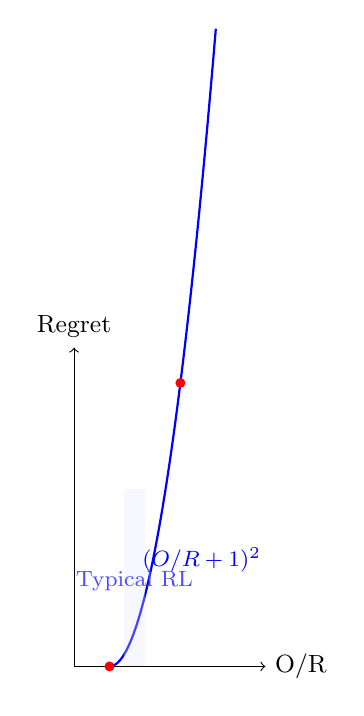
\begin{tikzpicture}[scale=0.9]
\draw[->] (-1.5,0) -- (1.2,0) node[right] {\small O/R};
\draw[->] (-1.5,0) -- (-1.5,4.5) node[above] {\small Regret};
\draw[thick, blue, domain=-1:0.5, smooth, samples=50] plot (\x, {(\x + 1)^2 * 4});
\fill[red] (-1, 0) circle (2pt);
\fill[red] (0, 4) circle (2pt);
\fill[blue!10, opacity=0.3] (-0.8, 0) rectangle (-0.5, 2.5);
\node[blue!70, font=\footnotesize] at (-0.65, 1.2) {Typical RL};
\node[blue, font=\footnotesize] at (0.3, 1.5) {$(O/R + 1)^2$};
\end{tikzpicture}
\caption{Coordination regret grows quadratically with O/R Index. Full analysis in Appendix~\ref{app:quadratic_proof}.}
\label{fig:quadratic_bowl}
\end{figure}

This bound provides theoretical support for using O/R as a coordination diagnostic and explains why CR-REINFORCE achieves +6.9\% improvement through O/R regularization. Full proof and implications in Appendix~\ref{app:quadratic_proof}.
